\documentclass[10pt,a4paper]{article}

\usepackage[
    a4paper,
    left=1cm,
    right=1cm,
    top=0.8cm,
    bottom=0.8cm
]{geometry}

\usepackage{enumitem}
\usepackage{titlesec}
\usepackage{hyperref}
\usepackage{tikz}
\usetikzlibrary{positioning,calc,arrows.meta}

\setlength{\parindent}{0pt}
\setlength{\parskip}{0pt}

\usepackage{draftwatermark}
\SetWatermarkText{This is a draft}    % the text shown
\SetWatermarkScale{3}           % size; reduce if it runs off the page
\SetWatermarkColor[gray]{0.8}     % 0 = black, 1 = white; higher is lighter
\SetWatermarkAngle{45}            % rotation in degrees (default is diagonal)
%\SetWatermarkLightness{0.9}       % alternative to the color command

\begin{document}

\begin{tikzpicture}[remember picture,overlay]
    \coordinate (A) at ([shift={(-0.6cm,-0.7cm)}]current page.north east);
    \coordinate (B) at ($(A) +(-4,-4)$);
    %\draw (A) rectangle (B);
    \node[inner sep=0pt] at ($(A)!0.5!(B)$)
        {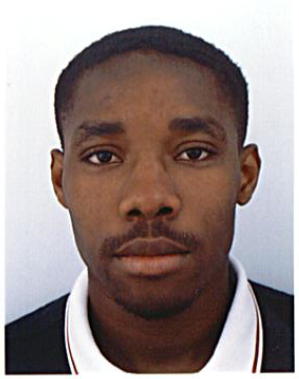
\includegraphics[width=4cm,height=4cm,keepaspectratio]{../ftc.png}};
\end{tikzpicture}
% ========================
%       YOUR CV
% ========================

\section*{Felix Touchte Codjo}
PhD student in particle physics

Université Paris-Saclay

IJCLab | Laboratoire de Physique des 2 Infinis Irène Joliot-Curie


\subsection*{\centering Profil}

Experimental physicist and engineer, I develop simulation and data reconstruction software within major international institutions (Jefferson Lab, IJCLab).
I'm contributor to the official reconstruction software (coatjava) of the CLAS collaboration and responsible for the development of the reconstruction code of the drift chamber of the new ALERT detector. I position myself at the crossroads of instrumentation, data analysis, and scientific software development, in the demanding context of experimental physics.
\#OpenToWorkInOctober2027

\section*{\centering Experience}

\subsection*{PhD Researcher}

\begin{minipage}{0.3\linewidth}
    IJCLab $\cdot$ Université Paris-Saclay
\end{minipage}
\begin{minipage}{0.4\linewidth}
    \raggedright
    Orsay, Île-de-France, France
\end{minipage}
\begin{minipage}{0.3\linewidth}
    \raggedleft
    October 2024 -- now
\end{minipage}

\begin{itemize}[label=$\circ$, itemsep=1pt]
    \item Member of the CLAS Collaboration
    \item Develop monitoring, reconstruction, and calibration codes for the ALERT experiment
    \item Measure the Coherent DVCS off $^4\mbox{He}$ with ALERT and CLAS at JLab
\end{itemize}

%Keywords: C/C++, Java, hadron structure, QCD, nuclear GPDs, DVCS, particle detection, data processing

\subsection*{Visiting Researcher}

\begin{minipage}{0.3\linewidth}
    Jefferson Lab
\end{minipage}
\begin{minipage}{0.4\linewidth}
    \raggedright
    Newport News, Virginia, The United States
\end{minipage}
\begin{minipage}{0.3\linewidth}
    \raggedleft
    March 2025 -- July 2025
\end{minipage}

\begin{itemize}[label=$\circ$, itemsep=1pt]
    \item Ensured the monitoring of the data during the run period
    \item Played the role of on-call detector expert for a 24/7 running accelerator
\end{itemize}

%Keywords: Data taking, monitoring, target change, target purge


\subsection*{Research Intern}

\begin{minipage}{0.3\linewidth}
    IJCLab
\end{minipage}
\begin{minipage}{0.4\linewidth}
    \raggedright
    Orsay, Île-de-France, France
\end{minipage}
\begin{minipage}{0.3\linewidth}
    \raggedleft
    March 2024 -- August 2024
\end{minipage}

\begin{itemize}[label=$\circ$, itemsep=1pt]
    \item Included the hit digitization of ALERT in the Geant4 simulation of CLAS
    \item Implemented the decoding algorithm
\end{itemize}

%Keywords: C/C++, Geant4, simulation, drift chamber, signal generation and processing

\subsection*{Engineering Intern}

\begin{minipage}{0.3\linewidth}
    CERN
\end{minipage}
\begin{minipage}{0.4\linewidth}
    \raggedright
    Geneva, Switzerland
\end{minipage}
\begin{minipage}{0.3\linewidth}
    \raggedleft
    May 2023 -- August 2023
\end{minipage}

\begin{itemize}[label=$\circ$, itemsep=1pt]
    \item Studied the linearity of the Outer Tracker for luminosity measurement during HL-LHC from simulation
    \item Studied the linearity of CMS luminometers with respect to the REMUS system
\end{itemize}

%Keywords: C/C++, ROOT, simulation, luminosity measurement, calibration

%Reference: https://indico.cern.ch/event/1313707/

% ========================
%       Education
% ========================

\section*{\centering Education}

\subsection*{Université Paris-Saclay}

\begin{minipage}{0.6\linewidth}
    Doctor of Philosophy - PhD, Elementary Particle Physics
\end{minipage}
\begin{minipage}{0.4\linewidth}
    \raggedleft
    October 2024 -- September 2027
\end{minipage}

\subsection*{Université de Strasbourg}

\begin{minipage}{0.6\linewidth}
    Master of Science - MS, Elementary Particle Physics
\end{minipage}
\begin{minipage}{0.4\linewidth}
    \raggedleft
    September 2023 -- June 2024
\end{minipage}

(Double degree with Télécom Physique Strasbourg)


\subsection*{Télécom Physique Strasbourg}

\begin{minipage}{0.6\linewidth}
    Engineering degree, Engineering Physics/Applied Physics
\end{minipage}
\begin{minipage}{0.4\linewidth}
    \raggedleft
    October 2021 -- September 2024
\end{minipage}

% \subsection*{CPGE Lycée National Léon Mba}

% \begin{minipage}{0.6\linewidth}
%     Higher school preparatory classes
% \end{minipage}
% \begin{minipage}{0.4\linewidth}
%     \raggedleft
%     September 2018 -- July 2021
% \end{minipage}

\vfill
\begin{center}
    Version date : \today
\end{center}


\end{document}